\svnid{$Id: rt_piping.tex 1 2015-08-30 15:39:28Z rodriqu_dd $}

\chapter{Piping\label{chap:piping}}

\section{Inleiding}
Dit hoofdstuk beschrijft de procedure om een piping berekening op te zetten en uit te voeren. 

\section{Toevoegen van een piping faalmechanisme}
\label{sec:addpiping}
Om een piping berekening uit te voeren, moet er allereerst een RT project aangemaakt zijn in het algemeen project. Een RT project wordt toegevoegd in het \textbf{Project} toolvenster. Door op het project met de rechter muisknop te klikken, en dan door voor de opties \textit{New} en vervolgens \textit{Item} te kiezen.

\begin{figure} [H]
	\centering
		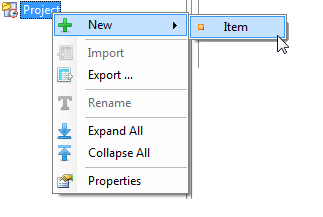
\includegraphics{figures/chapter_piping/addNewProject}
	\caption{Nieuw item toevoegen.}
	\label{fig:piping.addNewProject}
\end{figure}

In de dialoog die dan te zien is, moet er gekozen worden voor een RT project:

\begin{figure} [H]
	\centering
		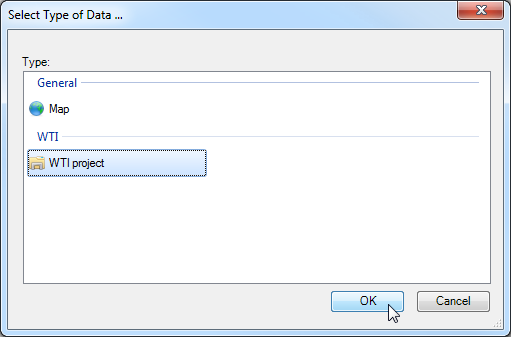
\includegraphics{figures/chapter_piping/selectRTProject}
	\caption{Nieuw toe te voegen item is RT project.}
	\label{fig:piping.selectRTProject}
\end{figure}

Door gebruik te maken van het contextmenu van het RT project, kan er uiteindelijk een piping faalmechanisme toegevoegd worden.

\begin{figure} [H]
	\centering
		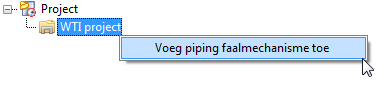
\includegraphics{figures/chapter_piping/addPipingMechanismToProject}
	\caption{Toevoeging van faalmechanisme Piping aan RT project.}
	\label{fig:piping.addPipingMechanismToProject}
\end{figure}

Het menu wordt nu uitgebreid met 3 onderdelen (zie \Fref{fig:piping.OpbouwFaalmechanisme}). De 2 onderdelen \textbf{Ondergrondprofielen} en \textbf{Dwarsdoorsneden} zijn nog niet gevuld en daarom in een lichtgrijze kleur weergegeven. Het onderdeel \textbf{Piping} is normaal van kleur, want hierin staan de standaard piping variabelen.

\section{Opbouw van het faalmechanisme}

\begin{figure} [H]
	\centering
		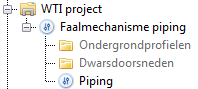
\includegraphics{figures/chapter_piping/OpbouwFaalmechanisme}
	\caption{Opbouw van het faalmechanisme}
	\label{fig:piping.OpbouwFaalmechanisme}
\end{figure}

Het faalmechanisme kent 3 onderdelen:
\begin{enumerate}
\item \textbf{Ondergrondprofielen}. Door gebruik te maken van het contextmenu (rechter muisknop) kan een .soil database met de stochastische schematisatie van de
ondergrond (SOS database) worden ge\"{i}mporteerd.
\item \textbf{Dwarsdoorsneden}. Door gebruik te maken van het contextmenu (rechter muisknop) kan een .csv database met de dwarsdoorsneden van het profiel (surfacelines) worden ge\"{i}mporteerd.\hfill \\

Als een onderdeel van \textbf{Ondergrondprofielen} of \textbf{Dwarsdoorsneden} is gevuld, wordt het item in een normale kleur weergegeven en staat er een plusteken voor de naam:

\begin{figure} [H]
	\centering
		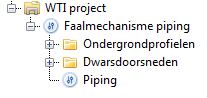
\includegraphics{figures/chapter_piping/FilledFailuremechanism}
	\caption{Gevulde onderdelen}
	\label{fig:piping.FilledFailuremechanism}
\end{figure}

Dit betekent dat het item kan worden uitgeklapt zodat alle profielen zichtbaar worden, en gekozen kunnen worden om te laten zien in het \textbf{Map venster}.

\begin{figure} [H]
	\centering
		\includegraphics{figures/chapter_piping/OpenFilledFailuremechanism}
	\caption{Geopende ondergrondprofielen}
	\label{fig:piping.openFilledFailuremechanism}
\end{figure}

\item \textbf{Piping}. In het \textbf{Properties} venster kunnen de piping varaiabelen worden aangepast:
\begin{figure} [H]
	\centering
		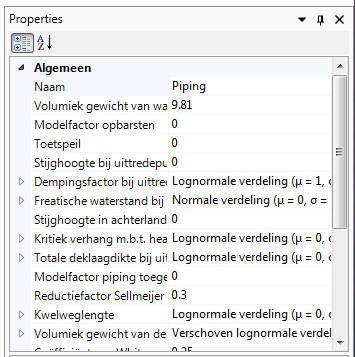
\includegraphics{figures/chapter_piping/PipingProperties}
	\caption{Aan te passen piping variabelen}
	\label{fig:piping.PipingProperties}
\end{figure}
	\begin{itemize}
	\item \textbf{Naam}: Naam van de berekening. Deze kan worden gewijzigd in het bijbehorende veld van het \textit{Properties} toolvenster, maar ook in het \textit{Project} toolvenster, door op de reeds geselecteerde piping berekening te klikken, of door \textbf{F2} erop te drukken.
	\item \textbf{Volumiek gewicht van water}: Het volumegewicht  $\gamma$ \textsubscript{water}  is ca. 10 kN/m\textsuperscript{3}
	\item \textbf{Modelfactor opbarsten}: Rekenwaarde van de modelonzekerheid
	\item \textbf{Toetspeil}: Het door HydraRing berekende toetspeil voor dit dijkvak
	\item \textbf{Stijghoogte bij uittredepunt}: 
	\item \textbf{Dempingsfactor bij uittredepunt}: Stochast; Relateert respons van stijghoogte bij binnenteen aan buitenwaterstand
	\item \textbf{Freatische waterstand bij uittredepunt}: Stochast; 
	\item \textbf{Stijghoogte in achterland}: 
	\item \textbf{Kritiek verhang m.b.t. heave}: Stochast; 
	\item \textbf{Totale deklaagdikte bij uittredepunt}: Stohast; Dikte van de laag boven de aquifer tot aan maaiveld of onderkant sloot
	\item \textbf{Modelfactor piping toegepast op Sellmeijermodel}: Rekenwaarde van de modelonzekerheid
	\item \textbf{Reductiefactor Sellmeijer}: 
	\item \textbf{Kwelweglengte}: De horizontale afstand tussen intrede- en uittredepunt die het kwelwater in de aquifer aflegt
	\item \textbf{Volumiek gewicht van de zandkorrels onder water}: Stochast; Het (ondergedompelde) volumegewicht van de korrels in de zandlaag.
	\item \textbf{Co\"{e}ffici\"{e}nt van White}: Sleepkrachtfactor volgens White
	\item \textbf{70\%-fraktiel van de korreldiameter in de bovenste zandlaag}: Stochast; Zeefmaat waar 70 gewichtsprocent van de korrels doorheen gaat. Hier de korreldiameter van het bovenste gedeelte van de aquifer, zonder de fijne fractie (<63$\mu$ meter)
	\item \textbf{Doorlatendheid aquifer}: Stochast; Darcy-snelheid waarmee water door de eerste zandlaag stroomt
	\item \textbf{Kinematische viscositeit van water bij 10\textsuperscript{$\circ$} Celsius}: 
	\item \textbf{Valversnelling}: Versnelling van de zwaartekracht [m/s\textsuperscript{2}] $\approx$ 9.81
	\item \textbf{Dikte watervoerend pakket}: Stochast; De dikte van de zandlaag die als aquifer is benoemd
	\item \textbf{Referentiewaarde voor 70\%-fraktiel in Sellmeijer regel}: Gemiddelde d70 van de in kleine schaalproeven toegepaste zandsoorten waarop de formule van Sellmeijer is gefit = 0.000208 meter
	\item \textbf{Rolweerstandshoek}: Hoek in het krachtenevenwicht die aangeeft hoeveel de korrels weerstand beiden tegen rollen; ook beddingshoek genoemd
	\begin{figure} [H]
	\centering
		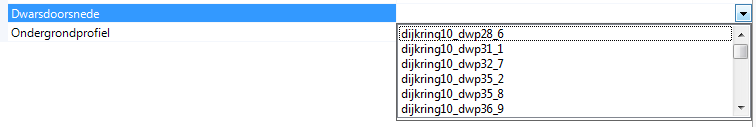
\includegraphics{figures/chapter_piping/PipingSurfacelines}
	\caption{Keuzemenu dwarsdoorsneden}
	\label{fig:piping.PipingSurfacelines}
\end{figure}
	\item \textbf{Dwarsdoorsnede}: Keuzemenu om de dwarsdoorsnede die voor de pipingsom wordt gebruikt te selecteren die zijn opgehaald in het \textbf{Project} venster
	\item \textbf{Ondergrondprofiel}: Keuzemenu om het ondergrondprofiel die voor de pipingsom wordt gebruikt te selecteren die zijn opgehaald in het \textbf{Project} venster
	\end{itemize}

\end{enumerate}


Er kunnen meerdere piping faalmechanismes berekeningen toegevoegd worden aan een \textit{Faalmechanisme piping} item. Deze optie is te vinden in het contextmenu van het \textit{piping faalmechanisme} (zie \textbf{(1)} in \Fref{fig:piping.validateAndRunPiping}).
Als alle invoergegevens voor een piping faalmechanisme berekening klaar zijn, kan het gecontroleerd worden of die berekening inderdaad uitgevoerd kan worden. Dit kan door \textit{Valideren} te kiezen in het contextmenu (zie \textbf{(3)} in \Fref{fig:piping.validateAndRunPiping}). Als er fouten gevonden worden tijdens de validatie waardoor de berekening niet uitgevoerd kan worden, is deze informatie terug te vinden in het bericht venster als foutmeldingen. Met behulp van de indicaties in deze berichten kunnen de benodigde aanpassingen in de berekening parameters ingevoerd worden. 
Wanneer een specifieke piping berekend kan worden (dit kan geconstateerd worden omdat er er geen foutmeldingen in het berichtvenster terechtkomen bij een validatie), kan de berekening daadwerkelijk uitgevoerd worden door op \textit{Berekenen} te klikken in het contextmenu van die specifieke berekening (zie \textbf{(4)} in \Fref{fig:piping.validateAndRunPiping}).
Het is ook mogelijk om alle berekeningen binnen een piping faalmechanisme item in één klap uit te voeren door \textit{Berekenen} te kiezen in het contextmenu van het faalmechanisme zelf dat die berekeningen bevat (zie \textbf{(2)} in \Fref{fig:piping.validateAndRunPiping}).

\begin{figure} [H]
	\centering
		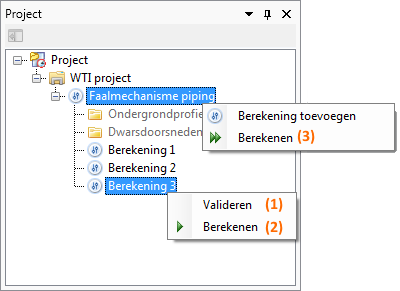
\includegraphics{figures/chapter_piping/validateAndRunPiping}
	\caption{Validatie en berekenen van piping faalmechanisme}
	\label{fig:piping.validateAndRunPiping}
\end{figure}


Als de berekening niet uitgevoerd kan worden, dan komt er een bericht terecht in het berichtpanel met verdere informatie over de reden dat het fout is gegaan. Als de berekening wel uitgevoerd is, is het resultaat toegevoegd (of ge\"{u}pdatet) in het projectpanel.





